\section {Konrad Ćwięka}
\label{sec:Konrad Ćwięka}

\subsection{Formulas }
Euler's number is a mathematical constant $ e = 2.71828$\\ It`s equal to: 
 \[e&=\lim_{n\to\infty}\left(1-\frac{1}{n}\right)^{n}\]
\subsection{Photo}
\begin{figure}[h]
    \centering
    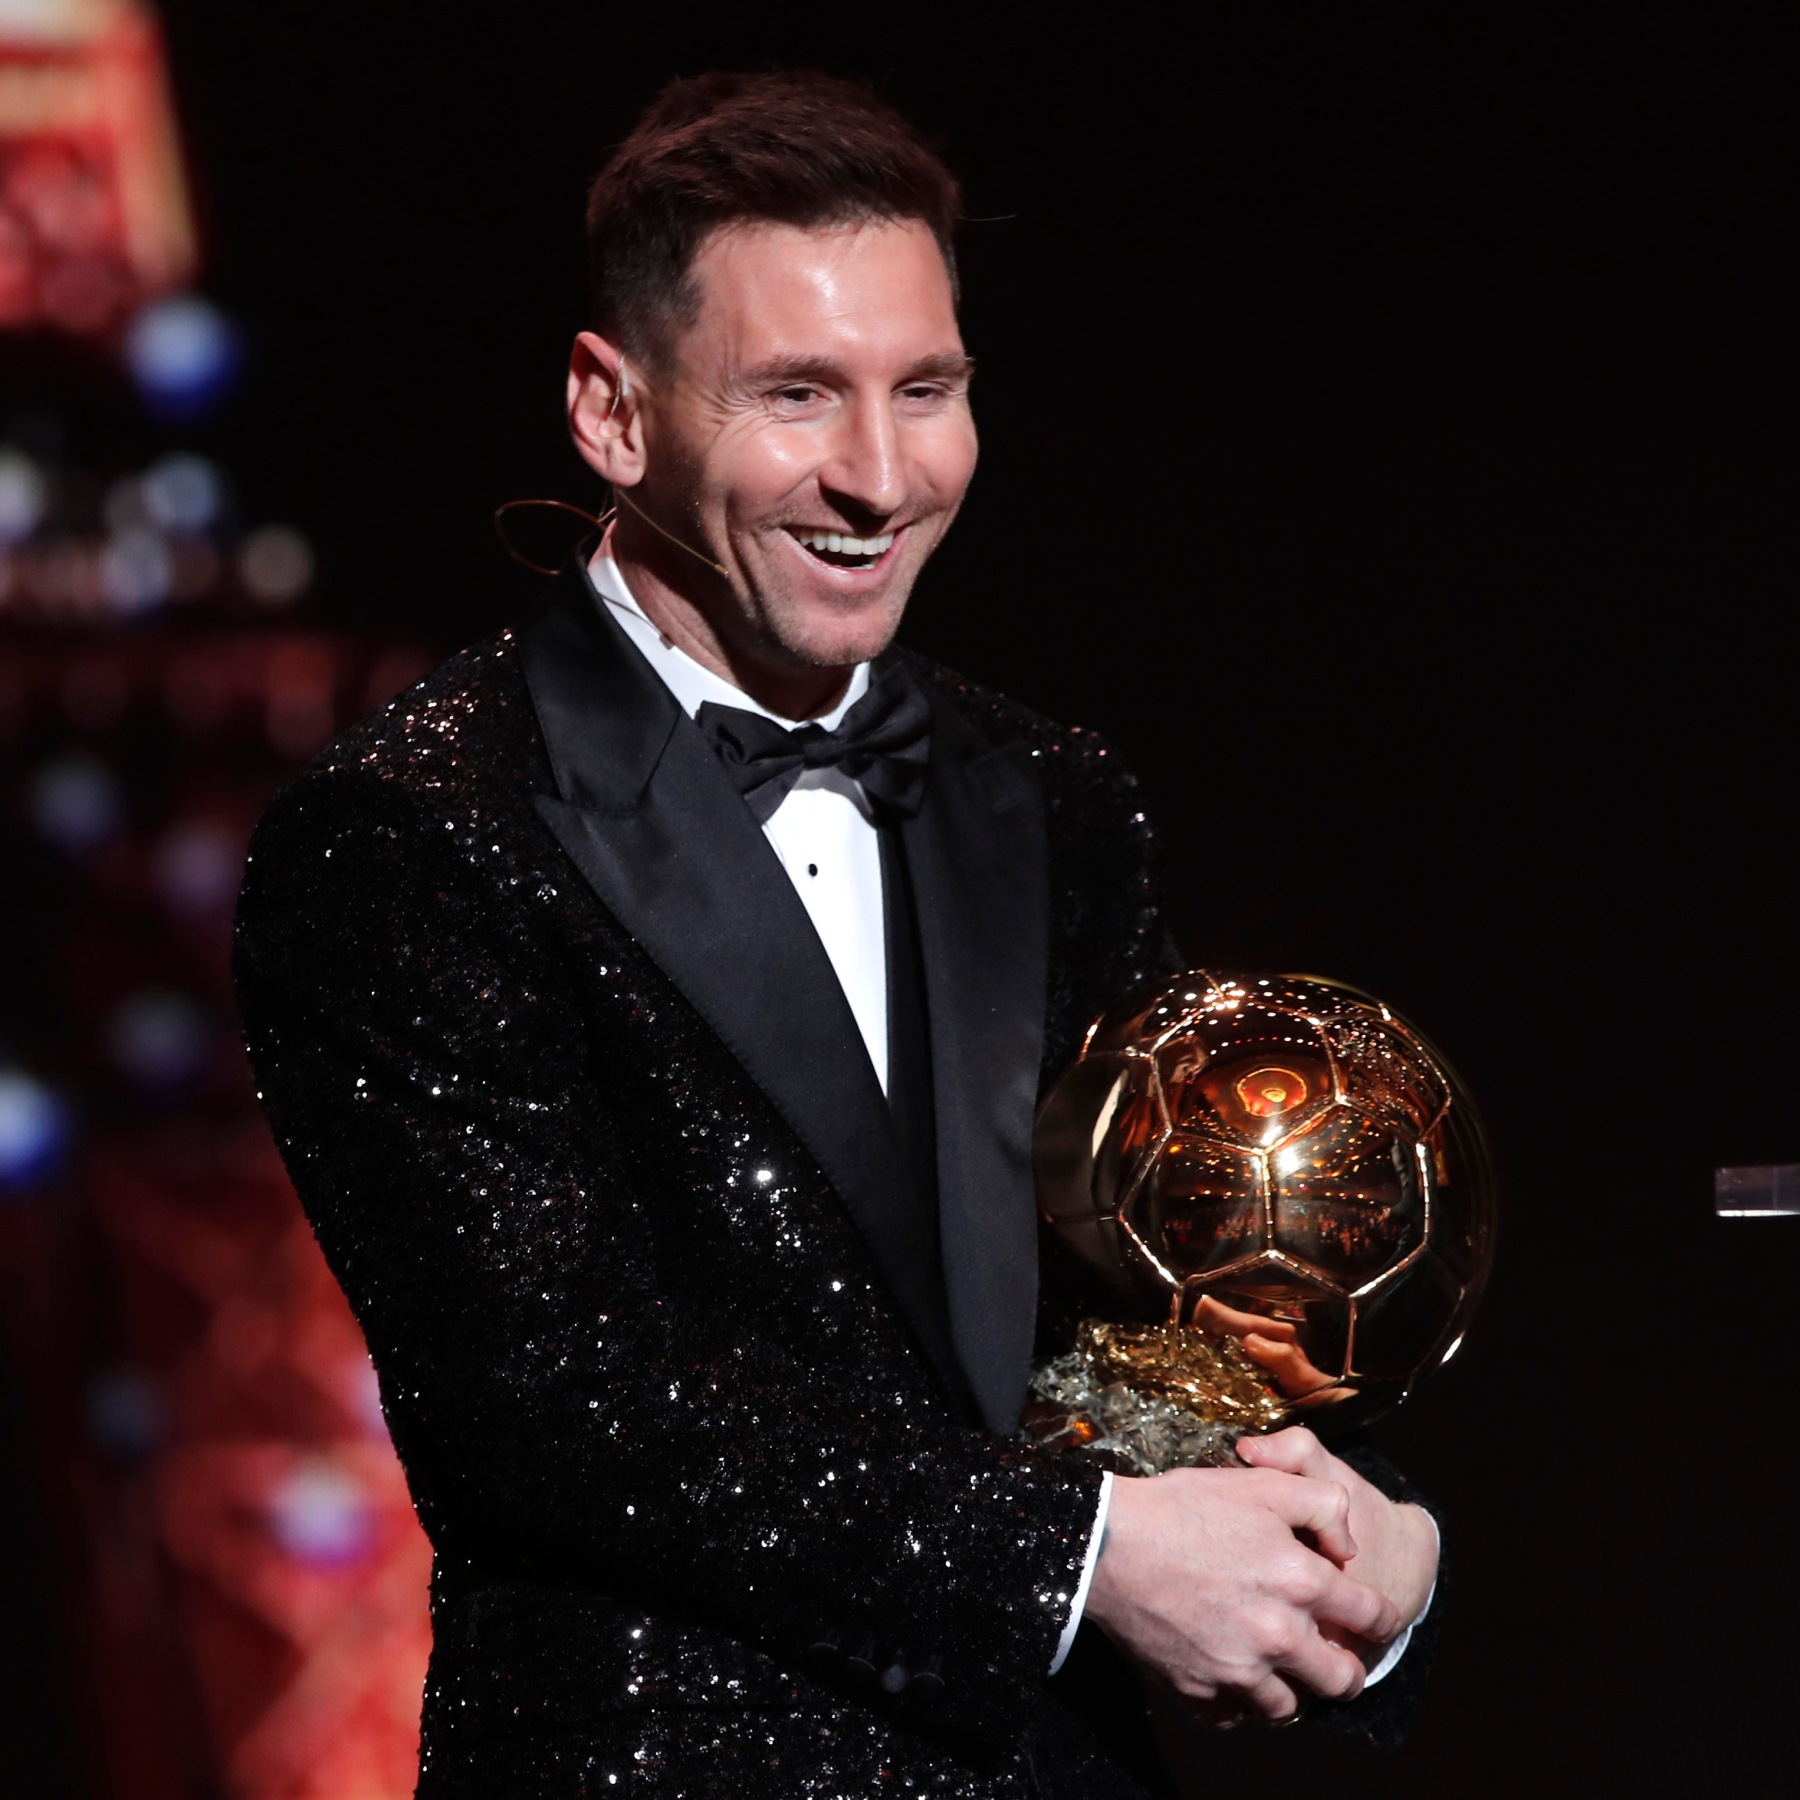
\includegraphics[scale = 0.2]{pictures/Ballon dor.jpg}
    \caption{Goat}
    \label{fig:Messi}
\end{figure}
\newpage
\subsection{Truth Table}
\begin{table}[h!]
\centering
\begin{tabular}{|c|c|c|c|c|c|c|}
\hline
\multicolumn{7}{|c|}{Truth Table}\\
\hline
\textbf{p} & \textbf{q} & \textbf{p$\land$ q} & \textbf{p$\lor$ q} & \textbf{$\neg$ p} & \textbf{p $\implies$ q} & \textbf{p $\iff$ q} \\ \hline
1          & 1          & 1                   & 1                  & 0                 & 1                       & 1                   \\ \hline
1          & 0          & 0                   & 1                  & 0                 & 0                       & 0                   \\ \hline
0          & 1          & 0                   & 1                  & 1                 & 1                       & 0                   \\ \hline
0          & 0          & 0                   & 0                  & 1                 & 1                       & 1                   \\ \hline
\end{tabular}
\end{table}

\renewcommand{\labelenumii}{\arabic{enumi}.\arabic{enumii}}

\subsection {Lista osiągnięć drużynowych: }
\begin{enumerate}
    \item \textbf{Mistrz świata} 
    \begin{enumerate}
        \item 2022 Argentyna
    \end{enumerate}
    \item \textbf{Zdobywca ligi mistrzów}
    \begin{enumerate}
        \item Barcelona 14/15
        \item Barcelona 10/11
        \item Barcelona 08/09
        \item Barcelona 05/06
    \end{enumerate}
    \item \textbf{Mistrz Hiszpani} 
    \begin{enumerate}
        \item Barcelona 18/19
        \item Barcelona 17/18
        \item Barcelona 15/16
        \item Barcelona 14/15
        \item Barcelona 12/13
    \end{enumerate}

\end{enumerate}
\subsection{Lista osiągnięć indywidualnych: }
\begin{itemize}
    \item \textbf{Zwycięzca Ballon d'Or}
    \begin{itemize}
        \item 2023
        \item 2021
        \item 2019
        \item 2015
    \end{itemize}
    \item \textbf{Król strzelców}
    \begin{itemize}
        \item Liga Mistrzów UEFA 18/19
        \begin{itemize}
            \item 12 bramek
        \end{itemize}
        \item LaLiga 12/13
        \begin{itemize}
            \item 46 bramek
        \end{itemize}
    \end{itemize}
\end{itemize}

\subsection{Biografia}
\setlength{\parindent}{20}
\par \textbf{Lionel Messi} urodził się \textit{24 czerwca 1987} w Rosario jako dziecko Jorge i Celii. Przygodę z piłką zaczął w wieku 5 lat, kiedy zapisał się do lokalnego klubiku Club Grandoli. Potem przeniósł się do Newell's Old Boys. Gdy miał 11 lat zdiagnozowano u niego \underline{karłowatość przysadkową}. Rodziny nie było stać na leczenie, ale pomocną dłoń wyciągnęła FC Barcelona, która zaprosiła Messich do Katalonii i zapłaciła za leczenie Leo. Jak się okazało był to strzał w dziesiątkę, bowiem Argentyńczyk z roku na rok stawał się coraz większą gwiazdą drużyn juniorskich, aż w końcu zadebiutował w seniorach. Dnia \textit{16 października 2004}roku Messi po raz pierwszy wystąpił w ligowym meczu FC Barcelony. Miał wtedy 17 lat i 114 dni. Minęło parę miesięcy i Argentyńczyk zdobył swojego pierwszego gola na hiszpańskich boiskach. Od tej pory trafiał już seryjnie. W międzyczasie zadebiutował również w Lidze Mistrzów, Katalończycy zmierzyli się wtedy z Udinese Calcio. \par
Z roku na rok \emph{Lionel Messi} stawał się coraz większą gwiazdą, a dziś śmiało można uznać go za najlepszego gracza mistrzów Hiszpanii. Najbardziej imponujące w jego wykonaniu okazały się być sezony \textbf{2008/2009, 2009/2010 i 2010/2011}. Wtedy bowiem Argentyńczyk rozegrał dla Blaugrany 159 spotkań, zdobywając w nich \underline{138 bramek}! W międzyczasie powiększył swoje konto o liczne strzeleckie trofea. \par
W dotychczasowej karierze klubowej Messi zdobył już praktycznie wszystko, co było do zdobycia. Był bowiem \textbf{pięciokrotnie mistrzem Hiszpanii, dwa razy wygrał Ligę Mistrzów, zdobywał także Puchar Hiszpanii, Superpuchar Hiszpanii, Superpuchar Europy i Klubowe Mistrzostwo Świata}.  Zdjęcie z najważniejszą piłkarską nagrodą indywidualną znajdziesz - \ref{fig:Messi}.